\section{Parsing}
\subsection{Derivazioni e Parsing}
Il \textbf{parsing} è il processo con cui, data una stringa, si verifica se essa appartiene al linguaggio generato da una grammatica, cercando di trovare una derivazione dalla radice (simbolo iniziale) fino alla stringa stessa. Si distinguono:
\begin{itemize}
    \item \textbf{Derivazione sinistra (leftmost):} si espande sempre la non-terminal più a sinistra.
    \item \textbf{Derivazione destra (rightmost):} si espande la più a destra.
\end{itemize}

\begin{tikzpicture}[
    level distance=2.5cm,
    sibling distance=4.2cm,
    grow=down,
    every node/.style={font=\large},
    edge from parent/.style={draw, -}
  ]
  \node {$E$}
    child { node {$T$}
      child { node {$F$}
        child { node {\underline{id}} }
      }
      child { node {$T'$}
        child { node {\underline{$\epsilon$}} }
      }
    }
    child { node {$E'$}
      child { node {\underline{+}} }
      child { node {$T$} [sibling distance=2cm]
        child { node {$F$}
          child { node {\underline{id}} }
        }
        child { node {$T'$} [sibling distance=1.2cm]
          child { node {\underline{*}} }
          child { node {$F$}
            child { node {\underline{id}} }
          }
          child { node {\underline{$\epsilon$}} }
        }
      }
      child { node {$E'$}
        child { node {\underline{$\epsilon$}} }
      }
    };
  \end{tikzpicture}
  
  

\subsection{Parser Top-Down}
Un \textbf{parser top-down} tenta di costruire una derivazione sinistra della stringa d’ingresso:
\begin{itemize}
    \item \textbf{Discesa ricorsiva:} implementazione semplice, tramite chiamate di procedura per ogni non-terminale.
    \item \textbf{Con backtracking:} prova tutte le produzioni possibili; torna indietro in caso di errore.
    \item \textbf{Senza backtracking (LL, tabellare):} per ogni \texttt{(stato, simbolo)} esiste una sola scelta.
\end{itemize}

\vspace{1em}
\begin{algorithm}
    \caption{Procedura di discesa ricorsiva per $A$}
    \begin{algorithmic}[1]
    \Procedure{A}{}
        \State Scegli, per $A$, una produzione $A \rightarrow X_1 X_2 \dots X_k$
        \For{ $i$ da $1$ fino a $k$ }
            \If{ $X_i$ è un non-terminale }
                \State richiama la procedura $X_i()$
            \ElsIf{ $X_i$ è uguale al simbolo d'ingresso corrente $a$ }
                \State procedi al simbolo successivo nella sequenza d'ingresso
            \Else
                \State /* si è verificato un errore */
            \EndIf
        \EndFor
    \EndProcedure
    \end{algorithmic}
    \end{algorithm}
    

\textbf{Esempio: per l'algoritmo della discesa ricorsiva}

Stringa da analizzare: \texttt{id + id * id}

% Tabella delle produzioni (puoi regolare ulteriormente la formattazione)
\begin{table}[ht]
    \centering
    \renewcommand{\arraystretch}{1.5}
    \begin{tabular}{|c|c|c|c|c|c|c|}
    \hline
    \textbf{Non} & \multicolumn{6}{c|}{\textbf{Simbolo d'ingresso}} \\
    \cline{2-7}
    \textbf{terminale} & \texttt{id} & \texttt{+} & \texttt{*} & \texttt{(} & \texttt{)} & \texttt{\$ (fine stringa)} \\
    \hline
    $E$  & $E \rightarrow T E'$     &             &             & $E \rightarrow T E'$ &             &             \\
    \hline
    $E'$ &                         & $E' \rightarrow +T E'$ &             &             & $E' \rightarrow \epsilon$ & $E' \rightarrow \epsilon$ \\
    \hline
    $T$  & $T \rightarrow F T'$     &             &             & $T \rightarrow F T'$  &             &             \\
    \hline
    $T'$ &                         & $T' \rightarrow \epsilon$ & $T' \rightarrow *F T'$ &             & $T' \rightarrow \epsilon$ & $T' \rightarrow \epsilon$ \\
    \hline
    $F$  & $F \rightarrow id$       &             &             & $F \rightarrow (E)$   &             &             \\
    \hline
    \end{tabular}
    \end{table}
\textit{La tabella guida le scelte dell'algoritmo in funzione del simbolo d'ingresso.}

\vspace{0.8em}
Produzioni:
\[
\begin{array}{l}
E \rightarrow T E' \\
T \rightarrow F T' \\
F \rightarrow id \\
T' \rightarrow * F T' \mid \epsilon \\
E' \rightarrow + T E' \mid \epsilon \\
\end{array}
\]

\vspace{0.8em}

Passaggi:
\begin{itemize}
    \item $E \rightarrow T E'$
    \item $T \rightarrow F T'$    \hspace{1em} (eseguo $F \rightarrow id$  $\Rightarrow$ \texttt{match()}, avanzo su "+")
    \item $T' \rightarrow \epsilon$
    \item $E' \rightarrow + T E'$  \hspace{1em} (match "+", avanzo su "id")
    \item $T \rightarrow F T'$     \hspace{1em} (match "id", avanzo su "\texttt{*}")
    \item $T' \rightarrow * F T'$  \hspace{1em} (match "*", avanzo su "id")
    \item $F \rightarrow id$       (match "id", arrivo a fine stringa)
    \item $T' \rightarrow \epsilon$
    \item $E' \rightarrow \epsilon$
\end{itemize}


\textbf{Esempio 2:}
\[
\begin{array}{l}
S \rightarrow cAd \\
A \rightarrow ab \mid a \\
S \rightarrow cAd \to c(ab)d \mid c(a)d
\end{array}
\]

Analisi:
\begin{enumerate}
    \item Input: \texttt{cad}
    \item Provo $A \rightarrow ab$\\
          \texttt{c} (\texttt{match}), \texttt{a} (\texttt{match}),\\
          \textbf{errore}: simbolo d'ingresso "d" non corrisponde a "b" $\Rightarrow$ backtracking
    \item Provo $A \rightarrow a$\\
          \texttt{c} (\texttt{match}), \texttt{a} (\texttt{match}), \texttt{d} (\texttt{match}), successo
\end{enumerate}

Nota: Le indentazioni non sono generalmente usate nell'approccio manuale della discesa ricorsiva.


\subsection{Parser Bottom-Up}
Nel \textbf{parser bottom-up} si parte dalla stringa e si cerca di ricostruire l’albero, risalendo fino al simbolo iniziale:
\begin{itemize}
    \item Ricerca una derivazione destra in maniera inversa (\emph{rightmost derivation in reverse}).
\end{itemize}

\subsection{Ricorsione Sinistra}
Se una grammatica presenta ricorsione sinistra (diretta o indiretta), cioè un non-terminale ha una regola di produzione che inizia con se stesso, la \textbf{discesa ricorsiva non funziona} senza modifiche:
\begin{itemize}
    \item \textbf{Ricorsione sinistra diretta:} Se la grammatica ha una produzione ricorsiva sinistra, ovvero:
        
\[
    S \rightarrow S \alpha \mid \beta
    \]
    
    allora la si può riscrivere eliminando la ricorsione sinistra come:
    
    \[
    \begin{cases}
    S \rightarrow \beta A \\
    A \rightarrow \alpha A \mid \varepsilon 
    \end{cases}
    \]

    Questa trasformazione può essere applicata anche in presenza di più ricorsioni sinistre nel sistema di produzioni.

    \item \textbf{Algoritmo di eliminazione:}
    \begin{enumerate}
        \item Ordina i non-terminali.
        \item Sostituisci produzioni ricorsive.
        \item Elimina la ricorsione immediata con una nuova variabile ausiliaria (A).
    \end{enumerate}

    \item \textbf{Ricorsione sinistra indiretta:} La ricorsione sinistra può essere \textbf{non diretta}.
    \end{itemize}       
    \subsection{Esempio di eliminazione della ricorsione sinistra non immediata}

    Consideriamo la grammatica:
    
    \[
    \begin{array}{l}
    S \rightarrow Aa \mid b \\
    A \rightarrow Ac \mid Sd \mid \varepsilon
    \end{array}
    \]
    
    \textbf{Primo passo:} si sostituiscono le occorrenze di $S$ nelle produzioni di $A$ usando la produzione di $S$, ottenendo:
    
    \[
    \begin{array}{l}
    S \rightarrow Aa \mid b \\
    A \rightarrow Ac \mid Aad \mid bd \mid \varepsilon
    \end{array}
    \]
    (Nota: sostituendo $S \to Aa$ in $Sd$, otteniamo $Aad$).
    
    \textbf{Secondo passo:} si identificano le parti ricorsive ($\alpha$) e le parti non ricorsive ($\beta$) per evidenziare la ricorsione sinistra diretta:
    
    \[
    \begin{array}{l}
    \text{Produzioni di } A: A \rightarrow A(c) \mid A(ad) \mid bd \mid \varepsilon \\
    \alpha_1 = c, \quad \alpha_2 = ad \\
    \beta_1 = bd, \quad \beta_2 = \varepsilon
    \end{array}
    \]
    
    \textbf{Terzo passo:} si elimina la ricorsione sinistra diretta da $A$ introducendo la variabile ausiliaria $A'$ e applicando la regola $A \to \beta A'$ e $A' \to \alpha A' \mid \varepsilon$:
    
    \[
    \begin{array}{l}
    S \rightarrow Aa \mid b \\
    A \rightarrow bd A' \mid A' \\
    A' \rightarrow c A' \mid ad A' \mid \varepsilon
    \end{array}
    \]
    (Nota: la produzione $A \to A'$ deriva da $\beta_2 A'$ dove $\beta_2 = \varepsilon$).
    
    In questo modo, la grammatica risultante è \textbf{priva di ricorsione sinistra} e adatta per un parser con discesa ricorsiva.

    Esiste un algoritmo sistematico per eliminare la ricorsione sinistra dalle grammatiche:


    \begin{algorithm}
        \caption{Eliminazione della ricorsione sinistra}
        \begin{algorithmic}[1]
        \State Ordina arbitrariamente i non-terminali come $A_1, A_2, \ldots, A_n$
        \For{ogni $i$ da $1$ fino a $n$}
            \For{ogni $j$ da $1$ fino a $i-1$}
                \State Sostituisci ogni produzione nella forma $A_i \rightarrow A_j \gamma$\\
                \hspace{1.5em}  con le produzioni $A_i \rightarrow \delta_1 \gamma \;|\; \delta_2 \gamma \;|\; \cdots \;|\; \delta_k \gamma$,\\
                \hspace{1.5em}  in cui $A_j \rightarrow \delta_1 \;|\; \delta_2 \;|\; \cdots \;|\; \delta_k$ sono tutte le produzioni per il non-terminale $A_j$ in esame
            \EndFor
            \State Elimina la ricorsione sinistra immediata dalle produzioni per $A_i$
        \EndFor
        \end{algorithmic}
    \end{algorithm}     

\textbf{Esempio 1:}
\[
\begin{array}{l}
A \rightarrow Ba \mid d \\
B \rightarrow Bb \mid Ac \mid \varepsilon \\
\end{array}
\]

\vspace{1em}
Dopo $i = 2$ (sostituzione di $A \rightarrow Ba$):
\[
\begin{array}{l}
A \rightarrow (Bb \mid Ac \mid \varepsilon) a \mid d \\[0.3em]
= Ba c \mid B b a \mid d a \mid d \\
B \rightarrow Bb \mid Ac \mid \varepsilon \\
\end{array}
\]

\vspace{1em}
Eliminando la ricorsione sinistra su $B$:

\[
\begin{array}{l}
A \rightarrow Ba \mid d \\
B \rightarrow dcB' \mid B' \\
B' \rightarrow bb' \mid acB' \mid \varepsilon \\
\end{array}
\]

\textbf{Esempio 2:}

\[
\begin{array}{l}
A \rightarrow Ba \mid C \\
B \rightarrow Cc \mid A \\
C \rightarrow Cc \mid d \\
\end{array}
\]

\vspace{1em}
Dopo sostituzioni:
\[
\begin{array}{l}
A \rightarrow Ba \mid C \\
B \rightarrow Cc \mid Ba \mid C \\
C \rightarrow Cc \mid d \\
\end{array}
\]

\vspace{1em}
Eliminando la ricorsione sinistra ($B$):

\[
\begin{array}{l}
A \rightarrow Ba \mid C \\
B \rightarrow CbB' \mid CB' \\
B' \rightarrow aB' \mid \varepsilon \\
C \rightarrow Cc \mid d \\
\end{array}
\]

\vspace{1em}
Eliminando la ricorsione sinistra ($C$):

\[
\begin{array}{l}
A \rightarrow Ba \mid C \\
B \rightarrow CbB' \mid CB' \\
B' \rightarrow aB' \mid \varepsilon \\
C \rightarrow dC' \\
C' \rightarrow cC' \mid \varepsilon \\
\end{array}
\]

\subsection{Fattorizzazione comune:}
Se $A \rightarrow \alpha\beta_1 \mid \alpha\beta_2 \mid \ldots \mid \alpha\beta_k \mid \gamma_1 \mid \gamma_2 \mid \ldots \mid \gamma_n$ \\
con $\alpha$ prefisso più lungo comune, allora si può riscrivere, raccogliendo per $\alpha$, come:

\[
\begin{aligned}
A &\rightarrow \alpha A' \mid \gamma_1 \mid \gamma_2 \mid \ldots \mid \gamma_n \\
A' &\rightarrow \beta_1 \mid \beta_2 \mid \ldots \mid \beta_k 
\end{aligned}
\]

\textbf{Esempio 1:}
\[
\begin{aligned}
A &\rightarrow abc d \mid abc e \mid abf \\
\end{aligned}
\]

\vspace{1em}
Fattorizzazione:
\[
\begin{aligned}
A &\rightarrow abc A' \mid abf \\
A' &\rightarrow d \mid e
\end{aligned}
\]

% oppure con doppio passaggio, come nell'immagine:
Oppure:
\[
\begin{aligned}
A &\rightarrow ab A'' \\
A'' &\rightarrow cA' \mid f \\
A' &\rightarrow d \mid e
\end{aligned}
\]


\textbf{Esempio 2: fattorizzazione comune + ricorsione diretta}

\[
\begin{aligned}
A &\rightarrow Abc d \mid Abc e \mid abf
\end{aligned}
\]

Fattorizzazione:
\[
\begin{aligned}
A &\rightarrow Abc A' \mid abf \\
A' &\rightarrow d \mid e
\end{aligned}
\]

Eliminazione ricorsione diretta:
\[
\begin{aligned}
A &\rightarrow abf A'' \\
A'' &\rightarrow bcA' A'' \mid \varepsilon \\
A' &\rightarrow d \mid e
\end{aligned}
\]

% oppure come nell'altra variante dell'immagine:
Oppure:
\[
\begin{aligned}
A &\rightarrow Abc d \mid Abc e \mid abf \\
\rightarrow abf A' \\
A' &\rightarrow bc d A'' \mid bc e A'' \mid \varepsilon \\
A'' &\rightarrow abf \mid cA'
\end{aligned}
\]



\subsection{Schema comparativo dei parser}

% Esempio di tabella comparativa
\begin{table}[h!]
\centering
\begin{tabular}{l|l|l}
Parser & Tecnica & Pro/Contro \\
\hline
Discesa ricorsiva & Top-down & Semplice, non sempre applicabile\\
LL(1), tabellare  & Top-down & Rapido, niente backtracking\\
Bottom-up (LR)    & Bottom-up & Più potente, tabellare\\
\end{tabular}
\end{table}

\subsection{FIRST e FOLLOW nelle Grammatiche Formali}
\subsection*{Definizione di FIRST}
\begin{itemize}
    \item L'insieme \textbf{FIRST} di un simbolo grammaticale (o stringa di simboli) indica i terminali che possono essere il primo simbolo derivato da quella variabile o sequenza.
    \item \textbf{Regole essenziali:}
    \begin{itemize}
        \item Se il simbolo è un terminale, \(\mathrm{FIRST}\) è il simbolo stesso.
        \item Se il simbolo è una variabile, si analizzano le produzioni possibili. Per ogni produzione, si aggiungono i simboli \(\mathrm{FIRST}\) derivabili dalle sottostringhe secondo le regole specifiche.
        \item Per una stringa \(X_1X_2\ldots X_n\) si applica una regola iterativa: si prende il \(\mathrm{FIRST}\) del primo simbolo non nullo e, se necessario, anche il \(\mathrm{FIRST}\) dei successivi se includono la produzione \(\varepsilon\) (vuota).
    \end{itemize}
\end{itemize}

\subsection*{Esempio di FIRST}
\begin{verbatim}
S → Ax | yB
B → zB
A → Ba | S
\end{verbatim}
\[
\mathrm{FIRST}(B) = \{z\}
\]
\[
\mathrm{FIRST}(A) = \{z, a\}
\]
\[
\mathrm{FIRST}(S) = \{y, x, z, a\}
\]

\subsection*{Definizione di FOLLOW}
\begin{itemize}
    \item L'insieme \textbf{FOLLOW} di una variabile raccoglie tutti i terminali che possono seguire quella variabile in qualche derivazione, includendo anche il marcatore di fine stringa se la variabile può essere l’ultima nel processo di derivazione.
    \item \textbf{Regole essenziali:}
    \begin{itemize}
        \item Si aggiunge il marcatore ``\$'' (fine stringa) a FOLLOW del simbolo di partenza.
        \item Se una variabile \(X\) può essere seguita da una stringa \(Y\), si aggiunge \(\mathrm{FIRST}(Y)\) a FOLLOW\((X)\).
        \item Se \(X\) è alla fine di una produzione, si aggiunge il FOLLOW della variabile precedente (Testa della Produzione).
    \end{itemize}
\end{itemize}

\subsection*{Esempio di FOLLOW}
\begin{verbatim}
S → ACB | Cbb | Ba
A → da | BC
B → g
C → h
\end{verbatim}
\[
\mathrm{FOLLOW}(S) = \{\$\}
\]
\[
\mathrm{FOLLOW}(A) = \{h, g, \$\}
\]
\[
\mathrm{FOLLOW}(B) = \{a, \$, h, g\}
\]
\[
\mathrm{FOLLOW}(C) = \{b, \$, g, h\}
\]


\subsection*{Calcolo di FIRST per una stringa}

Possiamo ora calcolare \textbf{FIRST} per una generica stringa \( X_1X_2\ldots X_n \) come segue. Si aggiungono a \(\mathrm{FIRST}(X_1X_2\cdots X_n)\) tutti i simboli di \(\mathrm{FIRST}(X_1)\) diversi da \( \varepsilon \).
Inoltre,
\begin{itemize}
    \item se \( \varepsilon \in \mathrm{FIRST}(X_1) \), si aggiungono a \(\mathrm{FIRST}(X_1X_2\cdots X_n)\) tutti i simboli (diversi da \( \varepsilon \)) di \(\mathrm{FIRST}(X_2)\);
    \item se \( \varepsilon \in \mathrm{FIRST}(X_2) \), si aggiungono tutti i simboli (diversi da \( \varepsilon \)) di \(\mathrm{FIRST}(X_3) \), e così via.
    \item Infine si aggiunge \(\varepsilon\) a \(\mathrm{FIRST}(X_1X_2\cdots X_n)\) se e solo se \(\varepsilon \in \mathrm{FIRST}(X_i)\) per ogni \( i \).
\end{itemize}

\subsection*{Regole per il calcolo di FOLLOW}
Per calcolare \(\mathrm{FOLLOW}(A)\) per tutti i non-terminali \(A\) si procede applicando le regole seguenti finché non sia più possibile aggiungere nulla all'insieme \textsf{FOLLOW}.

\begin{enumerate}
    \item Si aggiunga \$ a \(\mathrm{FOLLOW}(S)\), ricordando che \(S\) è il simbolo iniziale e \$ è il marcatore di fine della stringa d'ingresso.
    \item Se esiste una produzione del tipo \(A \rightarrow \alpha B \beta\), allora si aggiunga a \(\mathrm{FOLLOW}(B)\) ogni elemento di \(\mathrm{FIRST}(\beta)\) eccetto \( \varepsilon \).
    \item Se esiste una produzione del tipo \(A \rightarrow \alpha B\) oppure del tipo \(A \rightarrow \alpha B \beta\) per cui \(\mathrm{FIRST}(\beta)\) contiene \( \varepsilon \), allora tutti i simboli in \(\mathrm{FOLLOW}(A)\) appartengono anche a \(\mathrm{FOLLOW}(B)\).
\end{enumerate}

\subsection*{Esempio}
Facendo riferimento alla grammatica
\[
\begin{array}{rl}
E   &\rightarrow\ T\ E' \\
E'  &\rightarrow\ +\ T\ E'\ \mid\ \varepsilon \\
T   &\rightarrow\ F\ T' \\
T'  &\rightarrow\ *\ F\ T'\ \mid\ \varepsilon \\
F   &\rightarrow\ (E)\ \mid\ \mathrm{id} \\
\end{array}
\]
possiamo affermare:
\begin{enumerate}
  \item $\mathrm{FIRST}(F) = \mathrm{FIRST}(T) = \mathrm{FIRST}(E) = \{ (,\, \mathrm{id}  \}$.
  Per capire il perché, si noti che le due produzioni per $F$ hanno corpi che iniziano con i due simboli terminali $\mathrm{id}$ e parentesi aperta. $T$ ha una sola produzione il cui corpo inizia con $F$. Dato che $F$ non deriva $\varepsilon$, $\mathrm{FIRST}(T)$ deve coincidere con $\mathrm{FIRST}(F)$. Si ragiona poi allo stesso modo per $\mathrm{FIRST}(E)$.

  \item $\mathrm{FIRST}(E') = \{+,\, \varepsilon\}$. La ragione è che il corpo di una delle due produzioni per $E'$ inizia con il terminale $+$ e il corpo dell’altra è $\varepsilon$. Ogni volta che un non-terminale deriva $\varepsilon$, dobbiamo aggiungere $\varepsilon$ all’insieme $\mathrm{FIRST}$ di quel non-terminale.

  \item $\mathrm{FIRST}(T') = \{\ast,\, \varepsilon\}$. Il ragionamento è simile a quello visto per $\mathrm{FIRST}(E')$.

  \item $\mathrm{FOLLOW}(E) = \mathrm{FOLLOW}(E') = \{\text{)},\, \$\}$. Dato che $E$ è il simbolo iniziale, $\mathrm{FOLLOW}(E)$ deve contenere il simbolo speciale $\$$. La presenza del corpo $(E)$ spiega il perché la parentesi chiusa appartenga a $\mathrm{FOLLOW}(E)$. Per quanto riguarda $E'$, si nota che questo non-terminale appare sempre alla fine dei corpi delle produzioni per $E$. Ne consegue che $\mathrm{FOLLOW}(E')$ deve coincidere con $\mathrm{FOLLOW}(E)$.

  \item $\mathrm{FOLLOW}(T) = \mathrm{FOLLOW}(T') = \{+,\,\text{)},\, \$\}$. Si noti che $T$ appare nei corpi delle varie produzioni sempre seguito da $E'$. Ne consegue che ogni simbolo, a esclusione di $\varepsilon$, che appartiene a $\mathrm{FIRST}(E')$ deve appartenere anche a $\mathrm{FOLLOW}(T)$. Questo ragionamento spiega la presenza del simbolo $+$. Tuttavia, dato che $\mathrm{FIRST}(E')$ contiene $\varepsilon$ (cioè $E' \Rightarrow^* \varepsilon$) ed $E'$ è tutto ciò che segue $T$ nei corpi delle produzioni per $E$, tutti i simboli in $\mathrm{FOLLOW}(E)$ devono anche appartenere a $\mathrm{FOLLOW}(T)$. Questo spiega i simboli $\$$ e parentesi chiusa. Per quanto riguarda $T'$, si osserva che appare solo alla fine delle produzioni per $T$, si conclude che $\mathrm{FOLLOW}(T') = \mathrm{FOLLOW}(T)$.

  \item $\mathrm{FOLLOW}(F) = \{+,\, *,\,\text{)},\, \$\}$. Il ragionamento da seguire è analogo a quello per $T$, svolto al punto precedente.
\end{enumerate}

\subsection{Grammatiche LL(1)}

\subsection*{Definizione}
Una grammatica è detta \textbf{LL(1)} se:
\begin{itemize}
    \item Esiste sempre la possibilità di costruire un parser \textbf{top-down predittivo deterministico}, cioè un parser a discesa ricorsiva senza backtracking.
    \item La prima \textbf{L} indica che si analizza la stringa in ingresso da \emph{sinistra} verso destra (\textit{Left}).
    \item La seconda \textbf{L} indica che si costruisce una \emph{derivazione sinistra} (\textit{Leftmost derivation}).
    \item Il numero \textbf{1} indica che la regola da scegliere viene determinata guardando un solo simbolo \textit{lookahead}, cioè il prossimo simbolo della stringa in input.
\end{itemize}

\subsection*{Condizioni formali per le grammatiche LL(1)}

Una grammatica $G$ è \textbf{LL(1)} se e solo se soddisfa le seguenti condizioni per ogni variabile $A$:

Siano $A \rightarrow \alpha_1 \mid \alpha_2 \mid \dots \mid \alpha_k$ le produzioni per $A$, allora:

\begin{itemize}
    \item $\mathrm{FIRST}(\alpha_i) \cap \mathrm{FIRST}(\alpha_j) = \emptyset \quad\forall\, i \neq j$
    \item Se $\exists\, i$ tale che $\alpha_i \Rightarrow^* \varepsilon$, allora:
    \begin{itemize}
        \item $\alpha_j \not\Rightarrow^* \varepsilon \quad \forall\, j \neq i$
        \item $\mathrm{FOLLOW}(A) \cap \mathrm{FIRST}(\alpha_i) = \emptyset$
    \end{itemize}
\end{itemize}

\vspace{1em}

In modo equivalente, per ogni variabile:
\begin{itemize}
    \item Gli insiemi \textbf{FIRST} relativi alle parti destre delle produzioni sono due a due disgiunti.
    \item Esiste al più una parte destra che può derivare $\varepsilon$ e in questo caso l’insieme \textbf{FOLLOW} della variabile deve essere disgiunto dagli insiemi \textbf{FIRST} di tutte le parti destre, cioè dal \textbf{FIRST} della variabile.
\end{itemize}


\subsection*{Parsing a discesa ricorsiva per grammatiche LL(1)}

Il parsing a discesa ricorsiva LL(1) si implementa tipicamente come una funzione ricorsiva per ogni variabile non terminale. Dato $\alpha_i = X_1 X_2 \ldots X_n$, il codice generale è:

\begin{verbatim}
for (i = 1; i <= n; i++) {
    if (Xi è una variabile)
        Xi();
    else if (Xi == a)
        a = next.token;
    else
        errore();
}
\end{verbatim}


Dove:
\begin{itemize}
    \item $V$ è l'insieme dei simboli non terminali della grammatica (variabili).
    \item $a$ è il simbolo corrente dell’input (lookahead token).
    \item \texttt{next.token} restituisce il prossimo simbolo dell’input.
\end{itemize}

Questo schema viene adattato per ciascuna produzione della grammatica LL(1) durante la scrittura manuale di parser ricorsivi predittivi, consentendo di riconoscere la struttura dell'input senza backtracking.

\subsection*{Note Finali}
\begin{itemize}
    \item In presenza di conflitti (ricorsione sinistra, prefissi comuni), occorre riformulare la grammatica per adattarla a LL(1).
    \item Le grammatiche LL(1) sono fondamentali per costruire parser efficienti, semplici e deterministici.
\end{itemize}


\subsection{Tabelle di parsing predittivo LL(1)}

Le informazioni derivate dagli insiemi \textbf{FIRST} e \textbf{FOLLOW} di una grammatica possono essere raccolte in una \textbf{tabella di parsing predittivo} $M$. In questa tabella, le righe corrispondono alle variabili non terminali della grammatica, e le colonne ai terminali (più il marcatore di fine stringa $\$$). L’elemento $M[A, a]$ indica quale produzione applicare per espandere la variabile $A$ quando il simbolo corrente in ingresso è $a$.

\subsection*{Costruzione della tabella}
Per ogni produzione $A \rightarrow \alpha$ della grammatica $G$:
\begin{enumerate}
    \item Per ogni terminale $a \in \mathrm{FIRST}(\alpha)$, si mette $A \rightarrow \alpha$ in $M[A,a]$.
    \item Se $\varepsilon \in \mathrm{FIRST}(\alpha)$, allora per ogni simbolo $b \in \mathrm{FOLLOW}(A)$ (incluso eventualmente $\$$) si mette $A \rightarrow \alpha$ in $M[A,b]$.
    \item Se in $M[A, a]$ non c’è nessuna regola, si ha una condizione di errore: il simbolo $a$ non può essere derivato dalle produzioni di $A$.
    \item Se $M[A, a]$ contiene più di una regola allora la grammatica non è LL(1) (conflitto tra insiemi $\mathrm{FIRST}$ oppure $\mathrm{FOLLOW}$ e $\mathrm{FIRST}$).
\end{enumerate}

\subsection*{Esempio di tabella di parsing}

Per la grammatica
\[
\begin{array}{rl}
E   &\rightarrow\ T\ E' \\
E'  &\rightarrow\ +T E' \mid \varepsilon \\
T   &\rightarrow\ F T' \\
T'  &\rightarrow\ * F T' \mid \varepsilon \\
F   &\rightarrow\ (E) \mid \mathrm{id}
\end{array}
\]

Tabella di parsing LL(1):
\[
\begin{array}{c|cccccc}
    & \mathrm{id} & + & * & ( & ) & \$ \\
\hline
E   & E \rightarrow T E' &   &   & E \rightarrow T E' &   &   \\
E'  &   & E' \rightarrow +T E' &   &   & E' \rightarrow \varepsilon & E' \rightarrow \varepsilon \\
T   & T \rightarrow F T' &   &   & T \rightarrow F T' &   &   \\
T'  &   & T' \rightarrow \varepsilon & T' \rightarrow * F T' &   & T' \rightarrow \varepsilon & T' \rightarrow \varepsilon \\
F   & F \rightarrow \mathrm{id} &   &   & F \rightarrow (E) &   &   \\
\end{array}
\]

\subsection{Parsing predittivo non ricorsivo}
\begin{itemize}
    \item Lo stack iniziale contiene $\$$ (fondo) e il simbolo iniziale della grammatica.
    \item A ogni passo, il parser esamina il simbolo $X$ in cima allo stack e il simbolo di ingresso corrente $a$:
    \begin{itemize}
      \item \textbf{while} $X \neq \$\ $:
      \begin{itemize}
        \item \textbf{if} $(X = a)$ allora avanza il puntatore $ip$;
        \item \textbf{else if} $(X \in \Sigma \cup \{\$\})$ allora \textit{errore()};
        \item \textbf{else if} $(M[X, a] = \emptyset)$ allora \textit{errore()};
        \item \textbf{else if} $M[X, a] = X \to Y_1 Y_2 \ldots Y_k$ allora:
        \begin{itemize}
          \item produci come uscita $X \to Y_1 Y_2 \ldots Y_k$;
          \item inserisci $Y_k, Y_{k-1}, \ldots, Y_1$ nello stack (con $Y_1$ in cima);
        \end{itemize}
        \item assegna a $X$ il simbolo in cima allo stack $(X = \mathrm{pop}(P))$;
      \end{itemize}
      \item \textbf{if} $(a = \$)$ accetta; altrimenti \textit{errore()}.
    \end{itemize}
    \item Se lo stack contiene solo $\$$ e anche l’input contiene $\$$, l’input viene accettato.
\end{itemize}

\subsection*{Esempio di parsing passo-passo}
\begin{table}[h!]
  \centering
  \caption*{Parsing predittivo non ricorsivo (input: \texttt{id + id * id \$})}
  \renewcommand{\arraystretch}{1.1}
  \begin{tabular}{|l|l|l|l|}
  \hline
  \textbf{Riconosciuta} & \textbf{Stack}   & \textbf{Input}         & \textbf{Azione} \\ \hline
                        & $E\$$            & $id\ +\ id\ *\ id\$ $  &                 \\ \hline
                        & $TE'\$$           & $id\ +\ id\ *\ id\$ $  & output $E \to TE'$ \\ \hline
                        & $FT'E'\$$          & $id\ +\ id\ *\ id\$ $  & output $T \to FT'$ \\ \hline
  $id$                  & $T'E'\$$          & $+ id\ *\ id\$ $       & consuma $id$     \\ \hline
  $id$                  & $E'\$$            & $+ id\ *\ id\$ $       & output $T' \to e$ \\ \hline
  $id$                  & $+TE'\$$          & $+ id\ *\ id \$ $      & output $E' \to +TE'$ \\ \hline
  $id\ +$               & $TE'\$$           & $id\ *\ id\$ $         & consuma $+$      \\ \hline
  $id\ +$               & $FT'E'\$$          & $id\ *\ id\$ $         & output $T \to FT'$ \\ \hline
  $id\ + id$            & $T'E'\$$          & $*\ id\$ $             & consuma $id$     \\ \hline
  $id\ + id$            & $*FT'E'\$$        & $*\ id\$ $             & output $T' \to *FT'$ \\ \hline
  $id\ + id\ *$         & $FT'E'\$$         & $id\$ $                & consuma $*$      \\ \hline
  $id\ + id\ *$         & $idT'E'\$$        & $id\$ $                & output $F \to id$ \\ \hline
  $id\ + id\ *\ id$     & $T'E'\$$          & $\$$                   & consuma $id$     \\ \hline
  $id\ + id\ *\ id$     & $E'\$$            & $\$$                   & output $T' \to e$ \\ \hline
  $id\ + id\ *\ id$     & $ \$ $            & $\$$                   & output $E' \to e$ \\ \hline
  \end{tabular}
  
  \vspace{1ex}
  \textbf{NOTA:} $e$ indica la produzione vuota, cioè $e \equiv \varepsilon$
  \end{table}
  

\begin{table}[h!]
  \centering
  \caption*{Parsing predittivo non ricorsivo (input: \texttt{id * + id \$})}
  \begin{tabular}{|l|l|l|l|}
  \hline
  \textbf{Riconosciuta} & \textbf{Stack}      & \textbf{Input}     & \textbf{Azione} \\ \hline
                        & $E\$$             & $id\ *\ +\ id\ \$ $ &                \\ \hline
                        & $TE'\$$          & $id\ *\ +\ id\ \$ $ & output $E \rightarrow TE'$  \\ \hline
                        & $FTE'\$$         & $id\ *\ +\ id\ \$ $ & output $T \rightarrow FT'$  \\ \hline
                        & $idT'E'\$$       & $id\ *\ +\ id\ \$ $ & output $F \rightarrow id$   \\ \hline
  $id$                  & $T'E'\$$         & $*\ +\ id\ \$ $     & consuma $id$               \\ \hline
  $id$                  & $*FTE'\$$        & $*\ +\ id\ \$ $     & output $T' \rightarrow *FT'$ \\ \hline
  $id\ *$               & $FTE'\$$         & $+\ id\ \$ $        & consuma $*$                \\ \hline
  $id\ *$               & $FTE'\$$         & $+\ id\ \$ $        &                            \\ \hline
  \end{tabular}
  \end{table}
  
  \vspace{1ex}

  Questo tipo di tabella e parsing consente di implementare facilmente parser deterministici, garantendo l’assenza di backtracking quando la grammatica è LL(1).

\section*{Analisi Sintattica Bottom-Up}

I metodi bottom-up costruiscono l’albero di parsing partendo dalle foglie e procedendo verso l’alto fino alla radice.

\vspace{0.5em}
Esempio di grammatica:

\[
E \to T \mid E + T \quad,\quad
T \to F \mid T * F \quad,\quad
F \to id \mid (E)
\]

\vspace{1em}
Sequenze di parsing (esempio con simboli):

\begin{figure}[h]
    \centering
    % Configurazione stile alberi
    \tikzset{
        level distance=20pt,      % Distanza verticale tra i livelli
        sibling distance=5pt,     % Distanza orizzontale tra i nodi
        every node/.style={inner sep=1pt, font=\small},
        edge from parent/.style={draw, thin}
    }

    % --- Passo 1: Stringa iniziale (Livello 0) ---
    \begin{tikzpicture}[baseline=0cm]
        \node at (0,0) {\textbf{id} $*$ \textbf{id}};
        % Rettangolo invisibile per mantenere l'altezza coerente con gli altri
        \path (0,3); 
    \end{tikzpicture}
    \hfill
    % --- Passo 2: Riduzione id -> F (F sale a livello 1) ---
    \begin{tikzpicture}[baseline=0cm]
        % Albero F posizionato a y=20pt (Livello 1)
        \node at (0, 20pt) {F}
            child {node {\textbf{id}}};
        \node [right=0.2cm] at (0,0) {$*$ \textbf{id}};
        \path (0,3);
    \end{tikzpicture}
    \hfill
    % --- Passo 3: Riduzione F -> T (T sale a livello 2) ---
    \begin{tikzpicture}[baseline=0cm]
        % Albero T posizionato a y=40pt (Livello 2)
        \node at (0, 40pt) {T}
            child {node {F}
                child {node {\textbf{id}}}
            };
        \node [right=0.2cm] at (0,0) {$*$ \textbf{id}};
        \path (0,3);
    \end{tikzpicture}
    \hfill
    % --- Passo 4: Riduzione secondo id -> F ---
    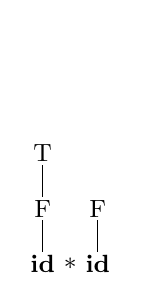
\begin{tikzpicture}[baseline=0cm]
        % Primo albero (T) fermo a livello 2
        \node at (0, 40pt) {T}
            child {node {F}
                child {node {\textbf{id}}}
            };
        % Simbolo * in basso
        \node at (0.35, 0) {$*$};
        % Secondo albero (F) a livello 1
        \node at (0.7, 20pt) {F}
            child {node {\textbf{id}}};
        \path (0,3);
    \end{tikzpicture}
    \hfill
    % --- Passo 5: Riduzione T * F -> T (Nuovo T sale a livello 3) ---
    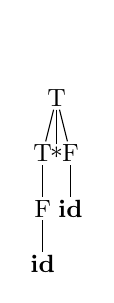
\begin{tikzpicture}[baseline=0cm]
        % Albero T risultante a y=60pt (Livello 3)
        \node at (0.35, 60pt) {T}
            child {node {T}
                child {node {F}
                    child {node {\textbf{id}}}
                }
            }
            child {node {$*$}}
            child {node {F}
                child {node {\textbf{id}}}
            };
        \path (0,3);
    \end{tikzpicture}
    \hfill
    % --- Passo 6: Riduzione T -> E (E sale a livello 4) ---
    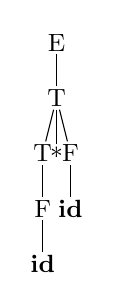
\begin{tikzpicture}[baseline=0cm]
        % Albero E finale a y=80pt (Livello 4)
        \node at (0.35, 80pt) {E}
            child {node {T}
                child {node {T}
                    child {node {F}
                        child {node {\textbf{id}}}
                    }
                }
                child {node {$*$}}
                child {node {F}
                    child {node {\textbf{id}}}
                }
            };
        \path (0,3);
    \end{tikzpicture}
\end{figure}

\vspace{2 cm}
Sequenze con somma:

\begin{figure}[h]
    \centering
    % Configurazione stile alberi
    \tikzset{
        level distance=20pt,      
        sibling distance=5pt,     
        every node/.style={inner sep=1pt, font=\small},
        edge from parent/.style={draw, thin}
    }

    % --- Passo 1: Stringa iniziale ---
    \begin{tikzpicture}[baseline=0cm]
        \node at (0,0) {\textbf{id}};
        \node at (0.35,0) {$+$};
        \node at (0.7,0) {\textbf{id}};
        \path (0,3); % Spazio verticale per allineamento
    \end{tikzpicture}
    \hfill
    % --- Passo 2: Primo id -> F ---
    \begin{tikzpicture}[baseline=0cm]
        \node at (0, 20pt) {F}
            child {node {\textbf{id}}};
        \node at (0.35,0) {$+$};
        \node at (0.7,0) {\textbf{id}};
        \path (0,3);
    \end{tikzpicture}
    \hfill
    % --- Passo 3: F -> T ---
    \begin{tikzpicture}[baseline=0cm]
        \node at (0, 40pt) {T}
            child {node {F}
                child {node {\textbf{id}}}
            };
        \node at (0.35,0) {$+$};
        \node at (0.7,0) {\textbf{id}};
        \path (0,3);
    \end{tikzpicture}
    \hfill
    % --- Passo 4: T -> E (Per preparare la somma E + T) ---
    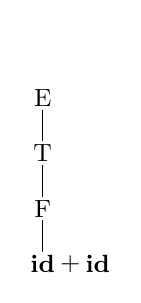
\begin{tikzpicture}[baseline=0cm]
        \node at (0, 60pt) {E}
            child {node {T}
                child {node {F}
                    child {node {\textbf{id}}}
                }
            };
        \node at (0.35,0) {$+$};
        \node at (0.7,0) {\textbf{id}};
        \path (0,3);
    \end{tikzpicture}
    
    \vspace{1cm} % Andiamo a capo per la seconda riga di passaggi
    
    % --- Passo 5: Secondo id -> F ---
    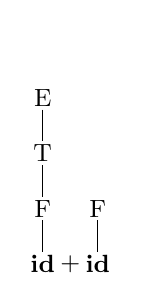
\begin{tikzpicture}[baseline=0cm]
        % Albero E a sinistra
        \node at (0, 60pt) {E}
            child {node {T}
                child {node {F}
                    child {node {\textbf{id}}}
                }
            };
        \node at (0.35,0) {$+$};
        % Albero F a destra
        \node at (0.7, 20pt) {F}
            child {node {\textbf{id}}};
        \path (0,3);
    \end{tikzpicture}
    \hfill
    % --- Passo 6: F -> T ---
    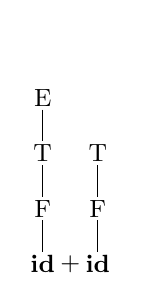
\begin{tikzpicture}[baseline=0cm]
        % Albero E a sinistra
        \node at (0, 60pt) {E}
            child {node {T}
                child {node {F}
                    child {node {\textbf{id}}}
                }
            };
        \node at (0.35,0) {$+$};
        % Albero T a destra
        \node at (0.7, 40pt) {T}
            child {node {F}
                child {node {\textbf{id}}}
            };
        \path (0,3);
    \end{tikzpicture}
    \hfill
    % --- Passo 7: Riduzione E + T -> E ---
    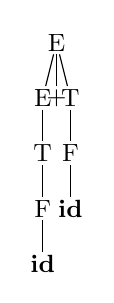
\begin{tikzpicture}[baseline=0cm]
        \node at (0.35, 80pt) {E}
            child {node {E}
                child {node {T}
                    child {node {F}
                        child {node {\textbf{id}}}
                    }
                }
            }
            child {node {$+$}}
            child {node {T}
                child {node {F}
                    child {node {\textbf{id}}}
                }
            };
        \path (0,3);
    \end{tikzpicture}
\end{figure}

Gli analizzatori bottom-up partono da una stringa \( w \) e procedono a ritroso, effettuando una progressiva riduzione fino ad ottenere il simbolo distinto \( S \).

\vspace{1em}
I parser bottom-up si basano sul meccanismo di riduzione che consiste nel sostituire la parte destra di una regola con la parte sinistra.

Una riduzione è l’inverso di un passo di derivazione, dove si espande una variabile con la parte destra di una regola, quindi un parser bottom-up ricostruisce in modo inverso una derivazione.

\vspace{1em}
Per gli esempi precedenti, considerando le radici dei sottoalberi, si hanno le sequenze di stringhe:

\[
id * id, \quad F * id, \quad T * id, \quad T * F, \quad T, \quad E,
\]

\[
id + id, \quad F + id, \quad T + id, \quad E + id, \quad E + F, \quad E + T, \quad E,
\]

corrispondenti alle derivazioni destre:

\[
E \Rightarrow T \Rightarrow T * F \Rightarrow T * id \Rightarrow F * id \Rightarrow id * id,
\]

\[
E \Rightarrow E + T \Rightarrow E + F \Rightarrow E + id \Rightarrow T + id \Rightarrow F + id \Rightarrow id + id.
\]

\vspace{1em}
Ad ogni passo, i parser bottom-up effettuano una riduzione oppure scandiscono un simbolo in ingresso. Per questo sono detti parser \textit{shift-reduce}, \textit{impila-riduci} o \textit{sposta-riduci}.

Le decisioni fondamentali sono se effettuare una riduzione e quale regola utilizzare.

Il parsing bottom-up scandisce una stringa da sinistra a destra e costruisce una derivazione destra.

Una \textbf{maniglia} (handle) è una sottostringa corrispondente alla parte destra di una regola la cui riduzione rappresenta un passo nella derivazione destra a ritroso.

\vspace{1em}
\textbf{Esempi di handle e regole di riduzione:}
\[
\begin{array}{lll}
\text{Forma di frase} & \text{Handle} & \text{Regola di riduzione} \\
\hline
id * id & id & F \to id \\
F * id & F & T \to F \\
T * id & id & F \to id \\
T * F & T * F & T \to T * F \\
T & T & E \to T \\
id + id & id & F \to id \\
F + id & F & T \to F \\
T + id & T & E \to T \\
E + id & id & F \to id \\
E + F & F & T \to F \\
E + T & E + T & E \to E + T \\
E & - & - \\
\end{array}
\]

\vspace{1em}
Nel primo esempio, nella stringa \( T * id \), \( T \) non viene ridotta anche se è parte destra della regola \( E \to T \).

Nel secondo esempio, nella stringa \( T + id \), \( T \) viene invece ridotta con la regola \( E \to T \).

Una sottostringa sinistra corrispondente alla parte destra di una regola non è necessariamente un handle.

Formalmente, se \( S \Rightarrow^{*} \alpha A w \Rightarrow \alpha \beta w \), la produzione \( A \to \beta \) nella posizione subito dopo \( \alpha \) è un handle di \( \alpha \beta w \).

\vspace{1em}
Un handle per una forma di frase destra \( \gamma \) è costituito dalla produzione \( A \to \beta \) e da una posizione in \( \gamma \) in cui si trova la stringa \( \beta \), tale che sostituendola con \( A \) si ottiene la forma di frase precedente in una derivazione destra di \( \gamma \).

In genere, con handle si intende la parte destra \( \beta \) della produzione.

La stringa \( w \) a destra dell’handle deve contenere solo simboli terminali: \( S \Rightarrow^{*} \alpha A w \Rightarrow \alpha \beta w \).

Se la grammatica è non ambigua, per ogni forma di frase destra c’è un unico handle.

Una derivazione destra può essere ottenuta a ritroso con un processo detto di \textit{potatura} o \textit{handle pruning}.

\newpage
\section*{Parsing Shift-Reduce}

Nel parsing \textit{impila-riduci} si usa uno stack che può contenere variabili e terminali, oltre al marcatore di fine stringa \( \$ \), e un buffer di ingresso che contiene la parte di input ancora da analizzare.

Un handle, subito prima di essere individuato, si trova sempre in cima allo stack.

Il simbolo \( \$ \) viene utilizzato come marcatore di fine stringa e per indicare il fondo dello stack. Inizialmente lo stack contiene \( \$ \) e in ingresso si ha \( w\$ \).

La stringa in ingresso viene scandita da sinistra a destra. Il parser inserisce nello stack (shift) zero o più simboli finché in cima non si trova un handle \( \beta \). A questo punto viene effettuata una riduzione (reduce) sostituendo \( \beta \) con la parte sinistra della regola opportuna.

Il parser ripete questo procedimento fino a rilevare un errore oppure quando lo stack contiene \( \$ S \) e in ingresso è rimasto solo \( \$ \).

\vspace{1em}
Ad ogni passo sono possibili 4 azioni:
\begin{enumerate}
    \item \textbf{Shift}: inserisce il prossimo simbolo in ingresso in cima allo stack.
    \item \textbf{Reduce}: il simbolo più a destra della stringa da ridurre si trova in cima allo stack. Si effettua una riduzione sostituendo la parte destra della regola con la parte sinistra.
    \item \textbf{Accept}: indica il corretto completamento dell’analisi.
    \item \textbf{Error}: si è verificata una situazione di errore.
\end{enumerate}

\vspace{1em}
Nell’esempio, lo stack viene rappresentato con l’elemento di testa a destra (così il contenuto dello stack e l’input da scandire, letti di seguito, corrispondono alle forme di frase destra).

\bigskip
\noindent\textbf{Esempio di parsing shift-reduce:}

\begin{table}[h!]
    \centering
    \begin{tabular}{|c|c|c|}
    \hline
    \textbf{Stack} & \textbf{Input} & \textbf{Azione} \\
    \hline
    \$ & \texttt{aaaaccbb\$} & \textit{shift} \\
    \$ a & \texttt{aaaccbb\$} & \textit{shift} \\
    \$ aa & \texttt{aaccbb\$} & \textit{shift} \\
    \$ aaa & \texttt{accbb\$} & \textit{shift} \\
    \$ aaaa & \texttt{ccbb\$} & \textit{shift} \\
    \$ \textcolor{teal}{aaaac} & \texttt{cbb\$} & \textit{reduce $A \to ac$} \\
    \$ aaaA & \texttt{cbb\$} & \textit{shift} \\
    \$ \textcolor{teal}{aaaAc} & \texttt{bb\$} & \textit{reduce $A \to aAc$} \\
    \$ aaA & \texttt{bb\$} & \textit{shift} \\
    \$ \textcolor{teal}{aaAb} & \texttt{b\$} & \textit{reduce $S \to aAb$} \\
    \$ aS & \texttt{b\$} & \textit{shift} \\
    \$ \textcolor{teal}{aSb} & \texttt{\$} & \textit{reduce $S \to aSb$} \\
    \$ S & \texttt{\$} & \textit{accept} \\
    \hline
    \end{tabular}
    \end{table}

Grammatica: 
\[
S \to aSb \mid aAb, \quad A \to aAc \mid ac
\]

\[
S \Rightarrow aSb \Rightarrow aaAbb \Rightarrow aaaAcbb \Rightarrow aaaaccbb
\]

\vspace{10 cm}
\subsubsection*{Esempio parsing shift-reduce con prodotto}

\begin{table}[h!]
    \centering
    \renewcommand{\arraystretch}{1.2}
    \begin{tabular}{|c|c|c|}
    \hline
    \textbf{Stack} & \textbf{Input} & \textbf{Azione} \\
    \hline
    \$ & \textbf{id * id \$} & \textit{shift} \\
    \textcolor{teal}{\$ id} & \textbf{* id \$} & \textit{reduce $F \rightarrow \textbf{id}$} \\
    \textcolor{teal}{\$ \textit{F}} & \textbf{* id \$} & \textit{reduce $T \rightarrow F$} \\
    \textcolor{teal}{\$ \textit{T}} & \textbf{* id \$} & \textit{shift} \\
    \textcolor{teal}{\$ \textit{T} *} & \textbf{id \$} & \textit{shift} \\
    \textcolor{teal}{\$ \textit{T} * id} & \textbf{\$} & \textit{reduce $F \rightarrow \textbf{id}$} \\
    \textcolor{teal}{\$ \textit{T} * \textit{F}} & \textbf{\$} & \textit{reduce $T \rightarrow T * F$} \\
    \textcolor{teal}{\$ \textit{T}} & \textbf{\$} & \textit{reduce $E \rightarrow T$} \\
    \textcolor{teal}{\$ \textit{E}} & \textbf{\$} & \textit{accept} \\
    \hline
    \end{tabular}
    \end{table}

\vspace{1em}

\subsubsection*{Esempio di parsing shift-reduce con somma:}

\begin{table}[h!]
    \centering
    \renewcommand{\arraystretch}{1.2}
    \begin{tabular}{|c|c|c|}
    \hline
    \textbf{Stack} & \textbf{Input} & \textbf{Azione} \\
    \hline
    \$ & \textbf{id + id \$} & \textit{shift} \\
    \textcolor{teal}{\$ id} & \textbf{+ id \$} & \textit{reduce $F \rightarrow \textbf{id}$} \\
    \textcolor{teal}{\$ F} & \textbf{+ id \$} & \textit{reduce $T \rightarrow F$} \\
    \textcolor{teal}{\$ T} & \textbf{+ id \$} & \textit{reduce $E \rightarrow T$} \\
    \textcolor{teal}{\$ E} & \textbf{+ id \$} & \textit{shift} \\
    \textcolor{teal}{\$ E +} & \textbf{id \$} & \textit{shift} \\
    \textcolor{teal}{\$ E + id} & \textbf{\$} & \textit{reduce $F \rightarrow \textbf{id}$} \\
    \textcolor{teal}{\$ E + F} & \textbf{\$} & \textit{reduce $T \rightarrow F$} \\
    \textcolor{teal}{\$ E + T} & \textbf{\$} & \textit{reduce $E \rightarrow E + T$} \\
    \textcolor{teal}{\$ E} & \textbf{\$} & \textit{accept} \\
    \hline
    \end{tabular}
    \end{table}
    
\vspace{1em}
L’uso dello stack è giustificato dal fatto che l’handle, a un certo punto, si trova sempre in cima allo stack, mai al suo interno.

Si può argomentare osservando due possibili casi per due passi successivi in una derivazione destra.

\vspace{1em}
\textbf{Caso 1:}
\begin{itemize}
    \item \( A \) è sostituito da \( \beta B y \)
    \item \( B \) (variabile più a destra in \( \beta B y \)) è sostituito da \( \gamma \)
\end{itemize}
La derivazione:

\[
S \Rightarrow^* \alpha A z \Rightarrow \alpha \beta B y z \Rightarrow \alpha \beta \gamma y z
\]

Letta a rovescio, quando il parser ha raggiunto la configurazione:

\[
\text{Stack: } \$ \alpha \beta \gamma \quad \text{Input: } y z \$
\]

Il parser riduce l’handle \( \gamma \) a \( B \) e ottiene:

\[
\$ \alpha \beta B \quad y z \$
\]

Poi può inserire \( y \) nello stack con una sequenza di zero o più shift, raggiungendo la configurazione:

\[
\$ \alpha \beta B y \quad z \$
\]

Con l’handle \( \beta B y \) in cima allo stack, che viene poi ridotto ad \( A \).

\vspace{1em}
\textbf{Caso 2:}
\begin{itemize}
    \item \( A \) è espanso sostituito da una stringa \( y \) di soli terminali
    \item \( B \) (variabile più a destra) si trova a sinistra di \( y \)
\end{itemize}
La derivazione:

\[
S \Rightarrow^* \alpha B x A z \Rightarrow \alpha B x y z \Rightarrow \alpha \gamma y z
\]

Nella configurazione:

\[
\$ \alpha \gamma \quad x y z \$
\]

L’handle \( \gamma \) è in cima allo stack. Dopo la riduzione di \( \gamma \) a \( B \), il parser inserisce \( x y \) nello stack, ottenendo in cima l’handle successivo da ridurre ad \( A \):

\[
\$ \alpha B x y \quad z \$
\]

\vspace{1em}
In entrambi i casi, dopo una riduzione, il parser deve fare zero o più shift per avere in cima allo stack l’handle successivo.

Il parser non deve mai analizzare l’interno dello stack per trovare l’handle.

\vspace{1 cm}
\textbf{Problema fondamentale nel parsing shift-reduce:} Quando in cima allo stack si ha una parte destra di una regola, come si fa a sapere se è un handle e quindi si deve fare la riduzione, oppure se è necessario ancora uno shift?

In cima allo stack potrebbero esserci parti destre di due regole diverse: quale si sceglie?

\vspace{10 cm}
\textbf{Esempio complesso di analisi:}


\begin{table}[h!]
    \centering
    \renewcommand{\arraystretch}{1.2}
    \begin{tabular}{|c|c|c|}
    \hline
    \textbf{Stack} & \textbf{Input} & \textbf{Azione} \\
    \hline
    \$ & \textbf{id + id * id \$} & \textit{shift} \\
    \textcolor{teal}{\$\;\textit{id}} & \textbf{+ id * id \$} & \textit{reduce $F \rightarrow $\textbf{id}} \\
    \textcolor{teal}{\$\;\textit{F}} & \textbf{+ id * id \$} & \textit{reduce $T \rightarrow F$} \\
    \textcolor{teal}{\$\;\textit{T}} & \textbf{+ id * id \$} & \textit{reduce $E \rightarrow T$} \\
    \textcolor{teal}{\$\;\textit{E}} & \textbf{+ id * id \$} & \textit{shift} \\
    \textcolor{teal}{\$\;\textit{E}+} & \textbf{id * id \$} & \textit{shift} \\
    \textcolor{teal}{\$\;\textit{E}+\,\textit{id}} & \textbf{* id \$} & \textit{reduce $F \rightarrow $\textbf{id}} \\
    \textcolor{teal}{\$\;\textit{E}+\,\textit{F}} & \textbf{* id \$} & \textit{reduce $T \rightarrow F$} \\
    \textcolor{teal}{\$\;\textit{E}+\,\textit{T}} & \textbf{* id \$} & \textit{shift} \\
    \textcolor{teal}{\$\;\textit{E}+\,\textit{T}*} & \textbf{id \$} & \textit{shift} \\
    \textcolor{teal}{\$\;\textit{E}+\,\textit{T}*\,\textit{id}} & \textbf{\$} & \textit{reduce $F \rightarrow $\textbf{id}} \\
    \textcolor{teal}{\$\;\textit{E}+\,\textit{T}*\,\textit{F}} & \textbf{\$} & \textit{reduce $T \rightarrow T * F$} \\
    \textcolor{teal}{\$\;\textit{E}+\,\textit{T}} & \textbf{\$} & \textit{reduce $E \rightarrow E + T$} \\
    \textcolor{teal}{\$\;\textit{E}} & \textbf{\$} & \textit{accept} \\
    \hline
    \end{tabular}
    \end{table}

\begin{table}[h!]
\centering
\renewcommand{\arraystretch}{1.2}
\begin{tabular}{|c|c|c|}
\hline
\textbf{Stack} & \textbf{Input} & \textbf{Azione} \\
\hline
\$ & \textbf{id + id + id \$} & \textit{shift} \\
\textcolor{teal}{\$\;\textit{id}} & \textbf{+ id + id \$} & \textit{reduce $F \rightarrow $\textbf{id}} \\
\textcolor{teal}{\$\;\textit{F}} & \textbf{+ id + id \$} & \textit{reduce $T \rightarrow F$} \\
\textcolor{teal}{\$\;\textit{T}} & \textbf{+ id + id \$} & \textit{reduce $E \rightarrow T$} \\
\textcolor{teal}{\$\;\textit{E}} & \textbf{+ id + id \$} & \textit{shift} \\
\textcolor{teal}{\$\;\textit{E}+} & \textbf{id + id \$} & \textit{shift} \\
\textcolor{teal}{\$\;\textit{E}+\,\textit{id}} & \textbf{+ id \$} & \textit{reduce $F \rightarrow $\textbf{id}} \\
\textcolor{teal}{\$\;\textit{E}+\,\textit{F}} & \textbf{+ id \$} & \textit{reduce $T \rightarrow F$} \\
\textcolor{teal}{\$\;\textit{E}+\,\textit{T}} & \textbf{+ id \$} & \textit{reduce $E \rightarrow E + T$} \\
\textcolor{teal}{\$\;\textit{E}} & \textbf{+ id \$} & \textit{shift} \\
\textcolor{teal}{\$\;\textit{E}+} & \textbf{id \$} & \textit{shift} \\
\textcolor{teal}{\$\;\textit{E}+\,\textit{id}} & \textbf{\$} & \textit{reduce $F \rightarrow $\textbf{id}} \\
\textcolor{teal}{\$\;\textit{E}+\,\textit{F}} & \textbf{\$} & \textit{reduce $T \rightarrow F$} \\
\textcolor{teal}{\$\;\textit{E}+\,\textit{T}} & \textbf{\$} & \textit{reduce $E \rightarrow E + T$} \\
\textcolor{teal}{\$\;\textit{E}} & \textbf{\$} & \textit{accept} \\
\hline
\end{tabular}
\end{table}



\section*{Parsing LR: concetti di base}
Il parsing usato comunemente per risolvere il problema è \textbf{LR(k)}:
\begin{itemize}
\item L (\textit{Left}): l’input viene letto da sinistra a destra.
\item R (\textit{Rightmost}): si costruisce una derivazione destra.
\item k: il parser può guardare i prossimi k simboli d’ingresso (di solito $k=1$).
\end{itemize}

\section*{Parsing LR: caratteristiche}
\begin{itemize}
    \item Si basa sulle tabelle di parsing.
    \item Una grammatica per la quale si può costruire la tabella si dice \textbf{LR}.
    \item Il parsing LR è adatto ai linguaggi di programmazione (grammatiche context-free).
    \item È il metodo shift-reduce più generale senza backtracking.
    \item Identifica errori sintattici appena possibile.
    \item Riconosce una classe più ampia delle grammatiche rispetto a LL.
\end{itemize}

\section*{Item LR(0) e stati}
Un parser LR prende le decisioni sposta/riduci memorizzando lo stato attuale.  
Ogni stato rappresenta un insieme di \emph{item}. Un \textbf{item LR(0)} di una grammatica $G$ è una produzione con un punto ($\cdot$) in una certa posizione della parte destra.  
Ad esempio, dato $A \to XYZ$ ci sono 4 item:
\begin{align*}
A &\to \cdot XYZ\\
A &\to X\cdot YZ\\
A &\to XY\cdot Z\\
A &\to XYZ\cdot
\end{align*}

La produzione $A \to \varepsilon$ genera solo $A \to \cdot$.

Ogni item indica che prefisso della produzione è già stato letto.

\section*{Significato degli item}
\begin{itemize}
    \item $A \to \cdot XYZ$: ci si aspetta in ingresso una stringa derivabile da $XYZ$.
    \item $A \to X\cdot YZ$: si sono riconosciuti simboli derivabili da $X$, ora ci si aspetta $YZ$.
    \item $A \to XYZ\cdot$: si è appena riconosciuta una stringa derivabile da $XYZ$, si può ridurre usando questa regola.
\end{itemize}

La \textbf{collezione canonica} LR(0) è un insieme di insiemi di item LR(0) e permette di costruire un automa a stati finiti deterministico (automa LR(0)), che serve per guidare le decisioni nel parsing.

\section*{Chiusura degli insiemi di item}
Per costruire la collezione canonica, si parte dalla grammatica aumentata $G'$, ottenuta introducendo $S' \to S$ per l’accettazione.

Sia $I$ un insieme di item di $G$. Definiamo la funzione di chiusura:
\begin{enumerate}
    \item Inizialmente $CLOSURE(I)$ contiene tutti gli item di $I$.
    \item Se $A \to \alpha \cdot B \beta$ è in $CLOSURE(I)$ e $B \to \gamma$ è una regola di $G$, si aggiunge $B \to \cdot \gamma$ (se non già presente). Si ripete finché non si aggiungono più item.
\end{enumerate}

\noindent\textbf{Esempio:}  
Grammatica aumentata:
\begin{equation*}
\begin{array}{l}
E' \to E \\
E \to E + T \mid T \\
T \to T * F \mid F \\
F \to (E) \mid id
\end{array}
\end{equation*}

Se $I = \{ [E' \to \cdot E] \}$, la $CLOSURE(I)$ conterrà:  
$E \to \cdot E + T$, $E \to \cdot T$, $T \to \cdot T * F$, $T \to \cdot F$, $F \to \cdot (E)$, $F \to \cdot id$.

Questa operazione di chiusura definisce il contenuto esatto del primo stato ($I_0$) dell'Automa LR(0) per la grammatica delle espressioni:

\[
\begin{array}{rcl}
E & \to & E + T \mid T \\
T & \to & T * F \mid F \\
F & \to & ( E ) \mid \mathbf{id}
\end{array}
\]
Partendo da questo stato iniziale, l'algoritmo calcola le transizioni (tramite la funzione \texttt{GOTO}) spostando il punto in avanti per ogni simbolo grammaticale. Ogni spostamento può generare un nuovo stato o portare a uno già esistente. 

Ripetendo questo processo iterativamente per tutti gli stati scoperti, si ottiene la \textbf{Collezione Canonica LR(0)}, visualizzata nel seguente Automa a Stati Finiti (DFA):

\vspace{1 cm}
\begin{figure}[H]
    \centering
    \begin{tikzpicture}[
        node distance=1.2cm and 1.5cm,
        box/.style={
            rectangle, 
            draw, 
            align=left, 
            font=\scriptsize,
            minimum width=1.8cm,
            inner sep=3pt,
            fill=white
        },
        arrow/.style={
            -Latex, 
            thick,
            rounded corners=3pt
        },
        label_edge/.style={
            pos=0.4,
            fill=white, 
            inner sep=1pt,
            font=\footnotesize\bfseries
        }
    ]

    % --- COLONNA PRINCIPALE (Sinistra) ---
    % I0: Stato Iniziale
    \node[box] (I0) {
        \textbf{I$_0$}\\
        $E' \to \cdot E$\\
        \color{gray}$E \to \cdot E + T$\\
        \color{gray}$E \to \cdot T$\\
        \color{gray}$T \to \cdot T * F$\\
        \color{gray}$T \to \cdot F$\\
        \color{gray}$F \to \cdot ( E )$\\
        \color{gray}$F \to \cdot \mathbf{id}$
    };

    % I2: Dopo aver letto T
    \node[box, below=1.8cm of I0] (I2) {
        \textbf{I$_2$}\\
        $E \to T \cdot$\\
        $T \to T \cdot * F$
    };

    % I4: Dopo aver letto '(' (Nodo centrale per ricorsioni)
    \node[box, below=1.8cm of I2] (I4) {
        \textbf{I$_4$}\\
        $F \to ( \cdot E )$\\
        \color{gray}$E \to \cdot E + T$\\
        \color{gray}... (closure)
    };

    % I3: Dopo aver letto F
    \node[box, below=1.8cm of I4] (I3) {
        \textbf{I$_3$}\\
        $T \to F \cdot$
    };

    % I5: Dopo aver letto id (Nodo centrale)
    \node[box] (I5) at ($(I2)!0.5!(I4)$) {
        \textbf{I$_5$}\\
        $F \to \mathbf{id} \cdot$
    };

    % --- COLONNA SUPERIORE (Dopo E) ---
    \node[box, right=2.5cm of I0] (I1) {
        \textbf{I$_1$}\\
        $E' \to E \cdot$\\
        $E \to E \cdot + T$
    };
    \node[below=0.2cm of I1, font=\bfseries] (acc) {accept};

    % --- COLONNA DESTRA (Dopo Operatori) ---
    
    % I6: Dopo E +
    \node[box, right=2.5cm of I1] (I6) {
        \textbf{I$_6$}\\
        $E \to E + \cdot T$\\
        \color{gray}$T \to \cdot T * F$\\
        \color{gray}$T \to \cdot F$\\
        \color{gray}...
    };

    % I7: Dopo T *
    \node[box, right=2.5cm of I2] (I7) {
        \textbf{I$_7$}\\
        $T \to T * \cdot F$\\
        \color{gray}$F \to \cdot ( E )$\\
        \color{gray}$F \to \cdot \mathbf{id}$
    };

    % I8: Dopo ( E
    \node[box, right=2.5cm of I4] (I8) {
        \textbf{I$_8$}\\
        $F \to ( E \cdot )$\\
        $E \to E \cdot + T$
    };

    % --- COLONNA ESTREMA DESTRA (Finali) ---
    
    % I9: Dopo E + T
    \node[box, right=2cm of I6] (I9) {
        \textbf{I$_9$}\\
        $E \to E + T \cdot$\\
        $T \to T \cdot * F$
    };

    % I10: Dopo T * F
    \node[box, right=2cm of I7] (I10) {
        \textbf{I$_{10}$}\\
        $T \to T * F \cdot$
    };

    % I11: Dopo ( E )
    \node[box, right=2cm of I8] (I11) {
        \textbf{I$_{11}$}\\
        $F \to ( E ) \cdot$
    };


    % --- COLLEGAMENTI ---

    % Da I0
    \draw[arrow] (I0) -- node[above] {E} (I1);
    \draw[arrow] (I1) -- (acc);
    \draw[arrow] (I0) -- node[left] {T} (I2);
    % Collegamenti lunghi da I0 a I4 e I5 usando percorsi a 'L'
    \draw[arrow] (I0.west) -- ++(-0.5,0) |- node[label_edge, near start] {(} (I4.west);
    \draw[arrow] (I0) |- node[label_edge, near end] {id} (I5); 
    % Nota: collegamento I0->I3 per F
    \draw[arrow] (I0.west) -- ++(-0.8,0) |- node[label_edge, near start] {F} (I3.west);

    % Da I1
    \draw[arrow] (I1) -- node[above] {+} (I6);

    % Da I2
    \draw[arrow] (I2) -- node[above] {*} (I7);

    % Da I4 (Il nodo più complesso)
    \draw[arrow] (I4) -- node[above] {E} (I8);
    \draw[arrow] (I4) edge[loop left] node[left] {(} (I4);
    \draw[arrow] (I4) -- node[left] {id} (I5);
    \draw[arrow] (I4) -- node[left] {T} (I2); % Risale a I2
    \draw[arrow] (I4) -- node[left] {F} (I3); % Scende a I3

    % Da I6 (Simile a I0 ma spostato)
    \draw[arrow] (I6) -- node[above] {T} (I9);
    % I6 verso id e (
    \draw[arrow] (I6.south) |- node[label_edge, near start] {id} (I5.east);
    \draw[arrow] (I6.south west) to[out=-135, in=45] node[label_edge] {(} (I4.north east);
    % I6 verso F -> I3 (Lungo giro)
    \draw[arrow] (I6.east) -- ++(0.5,0) |- node[label_edge, near start] {F} (I3.east);

    % Da I7
    \draw[arrow] (I7) -- node[above] {F} (I10);
    \draw[arrow] (I7) |- node[label_edge, near start] {id} (I5.east);
    \draw[arrow] (I7.south west) to[out=-135, in=20] node[label_edge] {(} (I4.north east);

    % Da I8
    \draw[arrow] (I8) -- node[above] {)} (I11);
    \draw[arrow] (I8) -- node[left] {+} (I6); % Risale per la somma

    % Da I9
    \draw[arrow] (I9) |- node[label_edge, near start] {*} (I7);

    \end{tikzpicture}
\end{figure}

\vspace{20 cm}

\section*{Algoritmi Closure e GOTO}
\textbf{Chiusura (pseudocodice):}
\begin{verbatim}
SetOfItems CLOSURE(I) {
    J = I
    repeat
        for (ogni item A -> alpha . B beta in J)
            for (ogni regola B -> gamma in G)
                if (B -> . gamma non in J)
                    aggiungi B -> . gamma a J;
    until nessun nuovo item è aggiunto a J;
    return J;
}
\end{verbatim}

\textbf{Funzione GOTO:}
Sia $I$ un insieme di item e $X$ un simbolo della grammatica,
\[
\mathrm{GOTO}(I, X) = \mathrm{CLOSURE}(\{ [A \to \alpha X \cdot \beta] \mid [A \to \alpha \cdot X \beta] \in I \})
\]
Usata per definire le transizioni dell’automa LR(0).

\section*{Collezione canonica LR(0)}
Costruita tramite:
\begin{verbatim}
void items(G') {
    C = CLOSURE({[S' -> .S ]});
    repeat
        for ( ogni insieme di item I in C )
            for ( ogni simbolo X in G )
                if (GOTO(I, X) non è vuoto e non appartiene a C )
                    aggiungi GOTO(I, X) a C;
    until nessun nuovo insieme di item è aggiunto a C;
}
\end{verbatim}
Gli stati dell’automa sono gli insiemi di item. La funzione di transizione è data da GOTO.

\section*{Parsing LR e la pila degli stati}

Durante il parsing si usa una tabella con più colonne:
\begin{itemize}
    \item Stack degli stati
    \item Stack dei simboli grammaticali
    \item Input residuo
    \item Azione (Shift, Reduce)
\end{itemize}
Ad ogni passo, se dallo stato $j$ c’è transizione col prossimo simbolo in ingresso $a$, allora si sceglie di impilare $a$. Altrimenti si effettua una riduzione.

\textbf{Quando si applica una riduzione $A \to X_1 X_2 \ldots X_n$}, si rimuovono $n$ stati dalla pila e si usa la funzione di transizione sull’ultimo stato rimasto e su $A$.

\section*{Esempio tabella di parsing}
\begin{table}[H]
    \centering
    \renewcommand{\arraystretch}{1.25}
    \begin{tabular}{|c|c|c|c|}
    \hline
    \textbf{Stack} & \textbf{Simboli} & \textbf{Input} & \textbf{Azione} \\
    \hline
    0 & $\$ $ & $\mathbf{id * id\ \$}$ & \textit{shift 5} \\
    0 5 & $\$\mathbf{id}$ & $\mathbf{* id\ \$}$ & \textit{reduce $F \rightarrow \mathbf{id}$} \\
    0 3 & $\$F$ & $\mathbf{* id\ \$}$ & \textit{reduce $T \rightarrow F$} \\
    0 2 & $\$T$ & $\mathbf{* id\ \$}$ & \textit{shift 7} \\
    0 2 7 & $\$T*$ & $\mathbf{id\ \$}$ & \textit{shift 5} \\
    0 2 7 5 & $\$T*\mathbf{id}$ & $\mathbf{\$}$ & \textit{reduce $F \rightarrow \mathbf{id}$} \\
    0 2 7 10 & $\$T*F$ & $\mathbf{\$}$ & \textit{reduce $T \rightarrow T * F$} \\
    0 2 & $\$T$ & $\mathbf{\$}$ & \textit{reduce $E \rightarrow T$} \\
    0 1 & $\$E$ & $\mathbf{\$}$ & \textit{accept} \\
    \hline
    \end{tabular}
    \end{table}
    
    L'esempio illustra le azioni del  parser shift-reduce durante l'analisi della stringa $\mathbf{id} * \mathbf{id}$, secondo l'automa LR(0), utilizzando uno stack per memorizzare gli stati dell'automa.

    Il processo si basa su due meccanismi principali:
    
    \begin{enumerate}
        \item \textbf{Lo Shift (Spostamento):}
        Quando lo stato in cima allo stack ha una transizione etichettata con il simbolo corrente in ingresso, il parser "sposta" il simbolo nello stack.
        \begin{itemize}
            \item \textit{Esempio:} All'inizio (linea 1), lo stack contiene lo stato iniziale \textbf{0}. Il simbolo in ingresso è $\mathbf{id}$. Poiché esiste una transizione $0 \xrightarrow{\mathbf{id}} 5$, il parser impila lo stato \textbf{5} (che corrisponde al simbolo $\mathbf{id}$).
        \end{itemize}
    
        \item \textbf{La Riduzione (Reduce):}
        Quando lo stato corrente non ha transizioni uscenti per il simbolo in ingresso, ma contiene un item completo (es. $F \to \mathbf{id} \cdot$), si effettua una riduzione.
        \begin{itemize}
            \item \textit{Esempio:} Alla linea 2, siamo nello stato \textbf{5} e l'input è $*$. Non ci sono transizioni uscenti, quindi si riduce usando $F \to \mathbf{id}$.
            \item \textbf{Meccanica della riduzione:}
            \begin{enumerate}
                \item Si rimuove dallo stack il corpo della produzione (in questo caso lo stato 5, corrispondente a $\mathbf{id}$).
                \item Lo stato che riemerge in cima è lo stato \textbf{0}.
                \item Si cerca la transizione dallo stato 0 sul simbolo testa della produzione ($F$). Poiché $0 \xrightarrow{F} 3$, si impila lo stato \textbf{3}.
            \end{enumerate}
        \end{itemize}
    \end{enumerate}
    
    Un comportamento analogo avviene successivamente (linea 5): partendo dallo stato \textbf{7} (che corrisponde al simbolo $*$), se arriva un $\mathbf{id}$ si fa shift verso lo stato 5. Successivamente, riducendo $F \to \mathbf{id}$, si rimuove il 5, riemerge il 7, e poiché $7 \xrightarrow{F} 10$, si impila lo stato \textbf{10}.
\section*{Nota}
Se nello stato 2, in cima alla pila, il prossimo simbolo è $*$, si effettua shift.
Se invece si facesse una riduzione, si rischierebbe di portare la macchina in errore.



